\documentclass[12pt,letterpaper]{article}
\usepackage[top=1in, bottom=1in, left=1in, right=1in]{geometry}
\usepackage{mfirstuc} %included to capatilize pronouns
\usepackage{subcaption}
\usepackage{wrapfig} % for wrapping text around a figure
\usepackage{tikz} %included for circuit diagrams
\usetikzlibrary{circuits.logic.US}
\usetikzlibrary{positioning}
\usepackage[hidelinks]{hyperref} % for final draft and print
%\usepackage{hyperref} % good for draft to see all references
\usepackage[all]{hypcap} % hyperlinks goto top of figures, not the bottom

\usepackage[capitalize,noabbrev,nameinlink]{cleveref}		% now \cref yields Figure 1.1 instead of 1.1 alone
												% must be included last due to its implementation.


\begin{document}

\author{Benjamin Viall}
\def\dateSubmitted{September 28, 2014}
\def\course {ECE 260: Digital Logic \& Coputer Design}
\def\lab{ Lab 1: An Introduction to Logic Circuits}
\def\dueDate{October 1, 2014}

\def\nameA{Ben Viall}
\def\nameB{Steve Shannon}
%\def\nameC{Patrick DaSilva}
%\def\nameD{Zaidan Shebar}

\def\TAGraded{} % comment this line if your lab is not graded by TA's


%ece260 specific definition for logical not
%\renewcommand*\lnot[1]{\overline{#1}} % better for long inversions.
\renewcommand*\lnot[1]{\bar{#1}} % better for single values


%%%%%%%%%%%%%%%%%%%%%%%%%%%%%%%%%%%%%%%%%%%%%%%%%%%%%%%%%%%%%%%%%%%%%%
%%% do not edit the title page unless you know what you are doing %%%%
%%%%%%%%%%%%%%%%%%%%%%%%%%%%%%%%%%%%%%%%%%%%%%%%%%%%%%%%%%%%%%%%%%%%%%

\begin{titlepage}

\center
\par 
\vfill

\hrulefill

\hrulefill

\LARGE\course

\Large\lab

\hrulefill
\def \possessive{my}
\def \pronoun{I}
\ifdefined\nameB 
 \def \possessive{our}
 \def \pronoun{we}	
\fi %nameB
\vfill
{\xmakefirstuc{\pronoun}} certify that this work is original and not a product of anyone's work but {\possessive} own.
\vskip .5in\nameA \hrulefill
\ifdefined\nameB
 \vskip .5in\nameB \hrulefill
\fi
\ifdefined\nameC
 \vskip .5in\nameC \hrulefill
\fi
\ifdefined\nameD
 \vskip .5in\nameD \hrulefill
\fi
\vfill
Submitted: \dateSubmitted

Due by: \dueDate

\vfill
\ifdefined\TAGraded
Graded by: \hrulefill
~~Date: \hrulefill
\fi
\end{titlepage}

\tableofcontents 
\clearpage
\listoffigures
\listoftables
\clearpage

%%%%%%%%%%%%%%%%%%%%%%%%%%%%%%%%%%%%%%%%%%%%%%%%%%%%%%%%%%%%%%%%%%%%
%%% Begin your lab report here %%%%%%%%%%%%%%%%%%%%%%%%%%%%%%%%%%%%%
%%%%%%%%%%%%%%%%%%%%%%%%%%%%%%%%%%%%%%%%%%%%%%%%%%%%%%%%%%%%%%%%%%%%
\begin{abstract}
In this lab the CADET workstation, DIP IC chips, and breadboard are introduced to students. A design task of creating a simple logic circuit is provided. To implement this circuit truth tables and boolean algebra are used to minimize the number of ICs required. The Fritzing software package is used to generate schematics and breadboard layout. Finally the cadet board is used to validate the built circuit.
\end{abstract}

\section{Introduction}
Digital logic is used in many levels of embedded design. Tt is important that both computer and electrical engineers have a firm grasp of the basic principals involved. This laboratory consists of three parts. In parts one and two, the use of the CADET Designer board is explained pictorially without the need to understand chip pin-outs. Part three consists of a design task that must:
\begin{itemize}
\item be analyzed
\item have a truth table generated
\item create and reduce logic equations 
\item create a schematic with part and pin numbers 
\end{itemize}

The schematic must then be transferred to a breadboard and verified to be working in front of the TAs or the instructor.


%\chapter{Body}
\section{Methods}
In this lab part one and two consisted of a step by step guide illustrating how to connect TTL chips to the cadet board to both stimulate the chips inputs, via logic switches, and observe the resulting output, via logic indicators. The procedure can be found in the lab folder on the engineering server. Part three involved designing a circuit based on a problem statement, implementing the circuit using TTL logic gates and verifying the behavior of the circuit.

\subsection{Part 1}
The 74LS08 quad 2 input AND gate was bread-boarded with a single gate connected to the cadet board as follows:
\begin{itemize}
\item pin 1: to logic switch 0
\item pin 2: to logic switch 1
\item pin 3: to logic indicator 0
\item pin 7: to ground
\item pin 14: to +5 volts
\item all other pins were left floating
\end{itemize}

The logic switches were toggled to the four possible combinations and the results recorded in tables.
A zero was used to indicate a switch in the low position and a one used to represent a switch in a high position. A zero in the results column indicates a red light while a one represents a green light.

After removing power from the circuit the 74LS08 was replaced with a 74LS00. The function of this chip was not given.  Powering the cadet board once again the logic switches were toggled and the results were recorded in another table. The process repeated again for an additional unknown chip 74LS32. 

With the 74LS32 chip still connected the wires were removed from pins one and two, the input pins, and the results recorded.


\begin{wraptable}{R}{0.6\textwidth}

\vspace{-50pt}
	\center
	\begin{tabular}{c c c | c || c c} 
	Q & D & N & \$ & beer & water \\
	\hline
	0 & 0 & 0 & 0 &0 &0  \\
	0 & 0 & 1 & 5 &0 &0  \\
	0 & 1 & 0 & 10&0 &0  \\
	0 & 1 & 1 & 15&1 &0  \\
	1 & 0 & 0 & 25&1 &0  \\
	1 & 0 & 1 & 30&1 &0  \\
	1 & 1 & 0 & 35&0 &1  \\
	1 & 1 & 1 & 40&0 &1  \\
\end{tabular}
\caption{Truth Table Generated For Part 3}
\label{fig:part3TT}
\end{wraptable}

\subsection{Part 2}

For the second part of the lab the breadboard was connected as shown in Illustration 4 in the lab handout. The two buttons were then pressed to record the outputs from all possible combinations of the buttons being pressed (P) and unpressed (U) and recorded in a table with the results column indicating 0 or 1 as in part one.

Next, pins one and two of the 74LS00 were connected together as shown in Illustration 5 of the lab handout; again the results of pressed and unpressed were recorded.

Lastly, the board was rewired as shown in illustration 6 of the lab handout, and the results of the logic switch vs indicator lights was recorded.

\subsection{Part 3}
\begin{figure}[ht]
\begin{center}
\begin{subfigure}{.4\textwidth}
\begin{center}
$beer=QD\lnot{N} + QDN$

$water= \lnot{Q}DN + Q\lnot{D}\lnot{N} + Q\lnot{D}N$
\end{center}

\caption{Un-Reduced}
\label{fig:part3unreduced}
\end{subfigure}
\begin{subfigure}{.4\textwidth}
\begin{center}
$beer=QD$

$water= \lnot{Q}DN + Q\lnot{D}$
\end{center}
\caption{Reduced}
\label{fig:part3reduced}
\end{subfigure}
\end{center}
\caption{Part 3 Equations}
\label{fig:equations}
\end{figure}


As prompted, a truth table was generated for all combinations of Quarters, Nickles, and Dimes. This table was augmented with the value of cash these combinations represented, simplifying the calculation of the two result columns as shown in \cref{fig:part3TT}.

From the truth table two un-reduced boolean algebra equations were then created, shown in \cref{fig:part3unreduced}. Using boolean algebra, these equations were reduced as shown in \cref{fig:part3reduced}. The next step was to create a logic schematic from the equations. Only AND, OR, and NOT gates were used as shown in \cref{fig:logicCircuits}.

\begin{figure}[ht!]
\begin{center}
	\begin{tikzpicture}[circuit logic US,minimum height=0.75cm] 
		\matrix[column sep=6mm]
		{
		\node (i0){Q};&                       &                      & & &\\
		              &                       &\node[and gate](g1){U2a};& & &\\
		\node (i1){D};& \node[not gate](g2){\ U3a\ };&                      & & &\\
		              &                       &                      &\node[or gate](g3){U4a}; & \node (o1){water}; & \\
		\node (i2){Q};& \node[not gate](g4){\ U3b\ };&                      & & \\ 
		\node (i3){D};&                       & \node[and gate US,draw,logic gate inputs=nnn] (g5) {U2b}; & & &\\
		\node (i4){N};&                       &                      & & &\\
		};
		
		
		\draw (i0.east) -- ++(right:3mm) |-  (g1.input 1);
		\draw (i1.east) -- ++(right:3mm) |-  (g2.input);
		\draw (i2.east) -- ++(right:3mm) |-  (g4.input);
		\draw (i3.east) -- ++(right:3mm) |-  (g5.input 2);
		\draw (i4.east) -- ++(right:3mm) |-  (g5.input 3);
		\draw (g1.output) -- ++(right:3mm) |-  (g3.input 1);
		\draw (g5.output) -- ++(right:3mm) |- (g3.input 2);
		\draw (g2.output) -- ++(right:3mm) |-  (g1.input 2);
		\draw (g4.output) -- ++(right:3mm) |- (g5.input 1);
		\draw (g3.output) -- (o1.west);
		

	\end{tikzpicture}
	\begin{tikzpicture}[circuit logic US,minimum height=0.75cm] 
	
	    \node[and gate,inputs=nnn] (g6){U2c};
	    \node[left=of g6.input 1] (i1){Q};
		\node[left=of g6.input 3] (i2){D};
		\node[right=of g6.output] (o1){beer};
		\draw (i1.east) -- (g6.input 1);
		\draw (i2.east) -- (g6.input 3);
		\draw (o1.west) -- (g6.output);
	
	\end{tikzpicture}
\end{center}
\caption{Logic Diagram For Beer and Water.}
\label{fig:logicCircuits}
\end{figure}

Too ensure that wiring was both simple to wire and simple to debug the schematic was then transferred to Fritzing .  By virtually reconfiguring the breadboard a simple circuit was derived and transferred to a real breadboard. Both the schematic and breadboard layout are available in the appendix.

Once the circuit had been built and brought into lab it was powered on. The test plan shown in \cref{fig:TestMatrix} was used to validate the function of the circuit. If the expected results matched the actual results in all cases the circuit was considered working.

\begin{table}
\center
\begin{tabular}{c c c  | c c | c c}
\multicolumn{3}{c|}{} & \multicolumn{2}{c|}{Expected} &\multicolumn{2}{c}{Actual} \\
Sw1 & Sw2 & Sw3 & Beer & Water & Beer & Water \\
\hline
0 & 0 & 0 &0 &0 & \multicolumn{2}{c}{}  \\
0 & 0 & 1 &0 &0 & \multicolumn{2}{c}{} \\
0 & 1 & 0 &0 &0 & \multicolumn{2}{c}{} \\
0 & 1 & 1 &1 &0 & \multicolumn{2}{c}{} \\
1 & 0 & 0 &1 &0 & \multicolumn{2}{c}{} \\
1 & 0 & 1 &1 &0 & \multicolumn{2}{c}{} \\
1 & 1 & 0 &0 &1 & \multicolumn{2}{c}{} \\
1 & 1 & 1 &0 &1 & \multicolumn{2}{c}{} \\

\end{tabular}
\caption{Test Matrix}
\label{fig:TestMatrix}
\end{table}


\section{Laboratory Experimental Results}

For this introductory lab experiment several chips were provided but the function of the 2 input gate inside the chip was not given. \Cref{fig:74xxResults} contains the results of the probing done in part one. A zero and one for the inputs indicates the logic switch in a lower or upper position respectively. A zero or one on the output indicates a green or red led lit respectively.

\begin{table}[ht]
	\begin{subtable}{.28\textwidth}
		\center
		\begin{tabular}{c c | c | c | c} 
		sw0 & sw1  & '08 & '00 & '32 \\
		\hline
		0 & 0 & 0 & 1 & 0\\
		0 & 1 & 0 & 1 & 1\\
		1 & 0 & 0 & 1 & 1\\
		1 & 1 & 1 & 0 & 1\\
	\end{tabular}
	\caption{74LSxx Chips}
	\label{fig:74xxResults}
	\end{subtable}
	\begin{subtable}{.36\textwidth}
		\center
		\begin{tabular}{c c | c} 
		s0 & s1  & 7400 \\
		\hline
		U & U & 0\\
		U & P & 1\\
		P & U & 1\\
		P & P & 1\\
		\end{tabular}
		\caption{74LS00 Using\\ Push-Buttons}
		\label{fig:buttonResults}
	\end{subtable}
	\begin{subtable}{.26\textwidth}
		\begin{center}
		\begin{tabular}{c | c} 
		sw0 & 7404 \\
		\hline
		P & 1\\
		U & 0\\
		\end{tabular}
		\end{center}	
		\caption{74LS04}
		\label{fig:inverterResults}
	\end{subtable}
	\caption{Recorded Values}
	\label{fig:RecordedValues}
\end{table}

For part two the 74LS00 was connected to push-buttons instead of logic switches. The question was 'Does a pressed button indicate a low logic or high logic state?'; therefore we recorded the results with U for unpressed and P for pressed; rather than with one's and zero's. The results are recorded in \cref{fig:buttonResults} and \cref{fig:inverterResults}. Comparing the two results tables we see that for the same chip the truth tables do not match up. this is important to answer the question posed in part 2: 'Does a pressed switch indicate a high or low condition?'.

\section{Discussion}
Throughout the lab questions were posed about why or how the circuit was exhibiting certain behaviors. In part one, several unidentified gates were provided. By testing all possible input combinations and comparing the results to truth tables of know functions we can determine that:
\begin{itemize}
\item a 74LS00 is a NAND gate
\item a 74LS08 is an AND gate
\item a 74LS32 is a OR gate
\end{itemize}

With a 74LS32 we were asked to disconnect both inputs and record the output. In our case the input stayed high even without any inputs. We must therefore conclude that the inputs on the OR gate "float" high when disconnected. It is important to remember that any input on a IC is interpreted as a HI or LO signal whether it is connected or not. Great care must be taken in future labs to ensure that all inputs are purposefully driven to some value. We can not assume that all gates will have their inputs float HI.

\begin{wraptable}{L}{.3\textwidth}
	\vspace{-20pt}
	\begin{center}
	\begin{tabular}{c c | c} 
	sw0 & sw1  & 7400 \\
	\hline
	P & P & 1\\
	P & U & 1\\
	U & P & 1\\
	U & U & 0\\
	\end{tabular}
	\end{center}
	\caption{Reordered Button Truth Table}
	\label{fig:reorderedButtons}
	\vspace{-10pt}
\end{wraptable}

In part two we connected an 74LS00 gate to push button switches on the cadet board using pull up resistors. In part one we have experimentally determined this to be a NAND chip. Comparing  \cref{fig:buttonResults} to \cref{fig:74xxResults} the the output columns should match up exactly, since it is the same chip. However, the outputs do not match up. When something does not work either you have done something wrong or you are working on false assumptions. In our case we assumed that when a button is unpressed it corresponded to a zero, so we wrote our truth table as UU,UP,PU,PP. If we reorder our truth table, as shown in \cref{fig:reorderedButtons}, we can see that the truth tables do exactly match. This leads us to the conclusion that a pressed button indicates a LO logic level. This is further enforced by examining the output of the 74LS04 inverter chip shown in \cref{fig:inverterResults}. When the button is pressed the result is a HI signal and when unpressed the result is a LO signal. since the output of an intverter is the oposite of the input we can once again see that the pressed state of a button is a LO logic level.

\section{Conclusions}
In this labratory we learned to use push buttons as inputs to logic gates. This will be important in later labs as we discovered it is faster to go through combinations of inputs using the buttons rather than the logic switches. Additionally, while we did not encounter any problems in generating our circuit we noticed problems that other groups had, and can now be wary of making similar mistakes in the future. These problems include but are not limited to:
\begin{itemize}
\item blowing up chips on power up. (solution check that no outputs are connected to any other outputs and be sure all chips are in the correct orientation.)
\item miss-wiring a circuit by a single row. (solution: check each wire at both ends before powering on circuit.)
\item blowing up chips while debugging. (solution: turn power off before making any changes to the circuit.)
\item logic LEDs not lighting either red or green (solution: while many causes exist, most likely there is a missing ground connection on a chip)
\item synthesizing the wrong circuit (solution: check with the professor or TA as soon as logic equations or truth table is generated)
\item keeping wires short, flat against the breadboard, and not going over chips makes probing and debugging easier.
\end{itemize}
Additionally, in a system with multiple outputs verify the functionality of each output separately. Several groups had a working "beer" circuit and a malfunctioning "water" circuit, but rewired both circuits rather than find the source of the problem. In this lab we learned to first take our logic schematic and write the expected state of all wires in the circuit based on the inputs that are causing incorrect outputs. Some errors are found at that point (i.e. the circuit that was designed is not correct). If the logic diagram disagrees with our experimental results we can then use a spare logic indicator to check the inputs of the last gate, compare the result to the annotated logic diagram and determine which input to that gate is faulty. We then trace the error back to its source. Most of the time it will be a mis-connected wire. We find errors either by getting a incorrect value (HI when we expect a LO) or getting no output on the led indicator lights.

\section{Laboratory Reflection}
In this laboratory experiment our problems did not arise out of a lack of ability to design or wire the circuit but in learning the tools. Fritzing is an interesting tool that speeds up breadboard development. We did have a head start by using the "bin" of parts provided by the professor. Unfortunately this package does not provide "logic" symbols, which led us to prepare our lab report using \LaTeX\ to generate the logic diagrams. \LaTeX\ however, has a VERY steep learning curve. Fortunately after preparing one lab report using this typesetting language the next labs should be much simpler, especially given the new \LaTeX\ template document that has been provided.

%\section{References}
\clearpage

\section{Appendix}
\ 
\begin{figure}[ht!]
\begin{center}
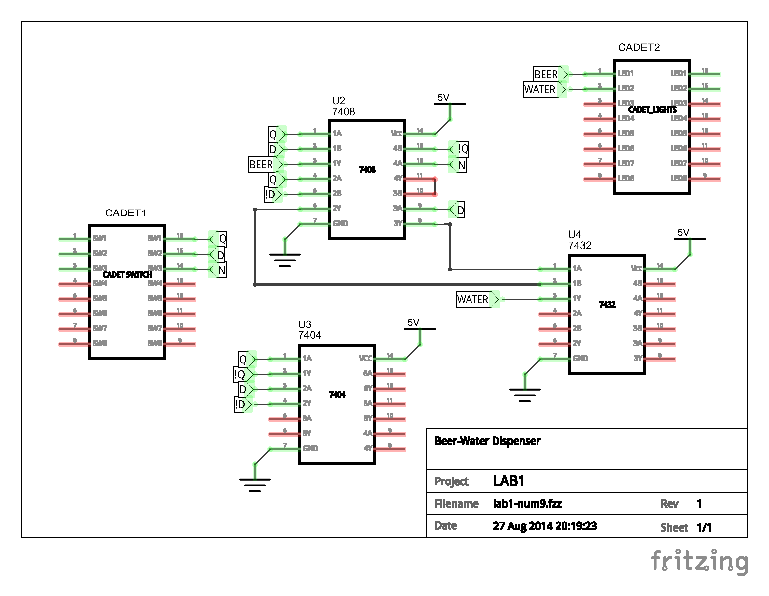
\includegraphics[scale=1,width=\textwidth]{lab1Images/lab1-num9_schem.pdf} 
\caption{Fritzing Schematic/Logic Schematic}
\label{fig:fritzSchematic}
\end{center}
\end{figure}

\begin{figure}[ht!]
\begin{center}
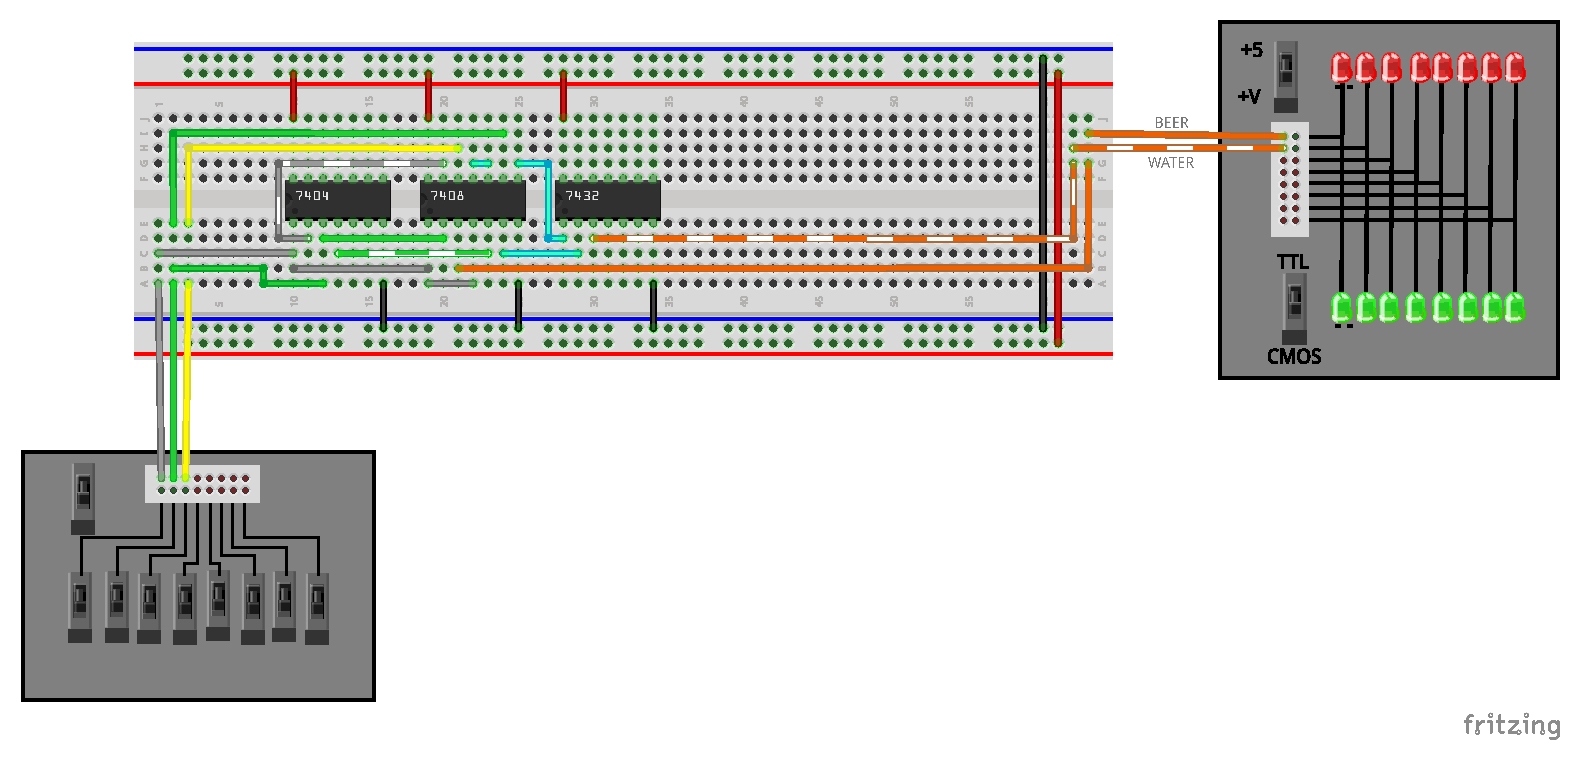
\includegraphics[angle=-90,scale=1,width=.5\textwidth]{lab1Images/lab1-num9_bb.pdf} 
\caption{Fritzing Breadboard}
\label{fig:fritzBreadboard}
\end{center}
\end{figure}


\end{document}
